%-------------------------------------------------------------------------%
\section{Decision Trees}

\begin{figure}[htbp]
    \centering
    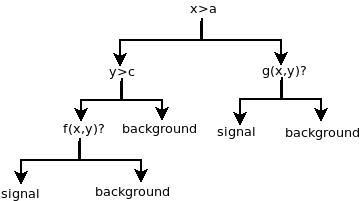
\includegraphics[width=10cm, height= 6cm]{DT.png}
    \caption{A simple decision tree for a hypothetical signal selection, expanding on Figure \ref{fig:cut} such that an extra parameter $g(x,y)$ is present within the algorithm.}
    \label{fig:tree}
\end{figure}

\begin{equation}
    f(x) = \sum_{i=1}^m c_m I(x\in R_m)
    \label{eq:DT}
\end{equation}

\begin{equation}
    G = \sum_{i=1}^K \hat{p}_k(1-\hat{p}_k)
    \label{eq:Gini}
\end{equation}

\begin{equation}
    S = -\sum_{i=1}^K \hat{p}_k \log(\hat{p}_k)
    \label{eq:Entropy}
\end{equation}

%-------------------------------------------------------------------------%
\section{Extreme Gradient Boosting - "xgboost"}


%-------------------------------------------------------------------------%